\newpage
{\bfseries IRSTI 31.15.15}

\sectionwithauthors{N. Akatyev}{SEMI-EMPIRICAL INVESTIGATION OF ZINC(II) SALICYLATE. COMPARISON
WITH X-RAY STRUCTURE.}

\begin{center}
{\bfseries N. Akatyev}

M.Utemisov West Kazakhstan university, Uralsk, Kazakhstan,

Corresponding author: nikolay.akatyev@wku.edu.kz
\end{center}

Zinc salicylate dihydrate
(Zn(HSal)\textsubscript{2}·2H\textsubscript{2}O) is an organic-inorganic
hybrid compound known for its wide range of applications. In this
article, a detailed semiempirical study of zinc salicylate is presented,
focusing on its structural, electronic, and thermodynamic properties.
The PM3 method, known for its computational efficiency and reasonable
accuracy, was used to model the molecular structure and compare with the
experimentally obtained properties of
Zn(HSal)\textsubscript{2}·2H\textsubscript{2}O. Based on the obtained
calculation results and available experimental data published in the
literature, it was found that semi-empirical calculations involving the
solvent effect (H\textsubscript{2}O) agree well with data from X-ray
diffraction analysis, while calculations for the gas phase do not agree
with experimental data with the required accuracy. Quantum chemical
descriptors such as HOMO-LUMO energies, energy gap
(ΔE\textsubscript{gap}), electronegativity (χ), global hardness (η),
softness (σ), dipole moment (μ), electrophilic (ω) and nucleophilic (ε)
indices were also calculated. The results show that the PM3 method
effectively captures the essential features of zinc salicylate,
including its geometry and electronic distribution. The obtained results
also provide valuable insights into the semi-empirical modeling of
organometallic compounds and highlight the usefulness of the PM3 method
in predicting the behavior of complex molecular systems.

{\bfseries Keywords:} PM3 calculations, zinc salicylate, semi-empirical
calculations, quantum chemical descriptors.

\begin{center}
{\large\bfseries МЫРЫШ(II) САЛИЦИЛАТЫН ЖАРТЫЛАЙ ЭМПИРИКАЛЫҚ ЗЕРТТЕУ. РЕНТГЕН
ҚҰРЫЛЫМЫМЕН САЛЫСТЫРУ.}

{\bfseries Н. Акатьев}

М.Өтемісов атындағы Батыс Қазақстан университеті, Орал, Қазақстан,

e-mail: nikolay.akatyev@wku.edu.kz
\end{center}

Мырыш салицилат дигидраты
(Zn(HSal)\textsubscript{2}·2H\textsubscript{2}O), қолдану аясының кең
ауқымымен танымал органикалық-бейорганикалық гибридті қосылыс. Бұл
мақалада оның құрылымдық, электронды және термодинамикалық қасиеттеріне
назар аудара отырып, мырыш салицилатының егжей-тегжейлі жартылай
эмпирикалық зерттеуі ұсынылған. Молекулярлық құрылымды модельдеу және
Zn(HSal)\textsubscript{2}·2H\textsubscript{2}O-ның тәжірибелік алынған
қасиеттерімен салыстыру үшін өзінің есептеу тиімділігі мен ақылға
қонымды дәлдігімен танымал PM3 әдісі қолданылды. Алынған есептеу
нәтижелеріне және әдебиетте жарияланған қолда бар эксперименттік
деректерге сүйене отырып, еріткіш әсерін (H\textsubscript{2}O) қамтитын
жартылай эмпирикалық есептеулер рентгендік дифракциялық талдау
деректерімен жақсы сәйкес келеді, ал газ фазасы үшін есептеулер сәйкес
келмейтіні анықталды. қажетті дәлдікпен эксперименттік деректермен.
HOMO-LUMO энергиясы, энергетикалық алшақтық (ΔE\textsubscript{gap}),
электртерістілік (χ), ғаламдық қаттылық (η), жұмсақтық (σ), дипольдік
момент (μ), электрофильдік (ω) және нуклеофильдік (ε) индекстері сияқты
кванттық химиялық дескрипторлар да болды. есептелген. Нәтижелер PM3
әдісі мырыш салицилатының маңызды ерекшеліктерін, соның ішінде оның
геометриясын және электрондық таралуын тиімді түрде түсіретінін
көрсетеді. Алынған нәтижелер сонымен қатар металлорганикалық
қосылыстардың жартылай эмпирикалық модельделуіне құнды түсініктер береді
және күрделі молекулалық жүйелердің әрекетін болжауда РМ3 әдісінің
пайдалылығын көрсетеді.

{\bfseries Түйін сөздер:} РМ3 есептеулері, мырыш салицилаты, жартылай
эмпирикалық есептеулер, кванттық химиялық дескрипторлар.

\begin{center}
{\large\bfseries ПОЛУЭМПИРИЧЕСКОЕ ИССЛЕДОВАНИЕ САЛИЦИЛАТА ЦИНКА(II). СРАВНЕНИЕ С
РЕНТГЕНОВСКОЙ СТРУКТУРОЙ.}

{\bfseries Н. Акатьев}

Западно-Казахстанский университет им.М.Утемисова, Уральск, Казахстан,

e-mail: nikolay.akatyev@wku.edu.kz
\end{center}

Дигидрат салицилата цинка
(Zn(HSal)\textsubscript{2}·2H\textsubscript{2}O)- гибридное
органо-неорганическое соединение, известное своим широким спектром
применения. В данной статье представлено подробное полуэмпирическое
исследование салицилата цинка с упором на его структурные, электронные и
термодинамические свойства. Для моделирования молекулярной структуры и
сравнения с экспериментально полученными свойствами
Zn(HSal)\textsubscript{2}·2H\textsubscript{2}O был использован метод
PM3, известный своей вычислительной эффективностью и приемлемой
точностью. На основании полученных расчётов и имеющихся
экспериментальных данных, опубликованных в литературе, установлено, что
полуэмпирические расчёты с учетом эффекта растворителя
(H\textsubscript{2}O) хорошо согласуются с данными рентгеноструктурного
анализа, тогда как расчеты для газовой фазы не согласуются с
экспериментальными данными с необходимой точностью. Были рассчитаны
квантово-химические дескрипторы, такие как энергии ВЗМО-НВМО,
энергетическая щель (ΔE\textsubscript{gap}), электроотрицательность (χ),
глобальная твердость (η), мягкость (σ), дипольный момент (μ),
электрофильные (ω) и нуклеофильные (ε) индексы. Результаты показывают,
что метод PM3 эффективно отражает основные характеристики салицилата
цинка, включая его геометрию и электронное распределение. Полученные
результаты также дают ценную информацию о полуэмпирическом моделировании
металлоорганических соединений и подчеркивают полезность метода PM3 для
прогнозирования поведения сложных молекулярных систем.

{\bfseries Ключевые слова:} PM3 расчёты, салицилат цинка, полуэмпирические
расчёты, квантово-химические дескрипторы.

\begin{multicols}{2}
{\bfseries Introduction.} Numerous branches of chemistry place significant
theoretical and practical emphasis on the structure and characteristics
of transition metal salicylates. These simple organic salts of salicylic
acid (\emph{o}-hydroxybenzoic acid) have a wide range of applications
because of their beneficial qualities. Compounds with carboxyl groups
are intriguing from the standpoint of coordination chemistry because
they can bind to metal ions as mono-, bi-, and bridging ligands.

Over the last two decades, a wide range of transition metal complexes
containing salicylate and its various derivatives have been described.
Das \emph{et al.} reported a highly porous and thermally stable Co(II)
salicylate metal--organic framework (MOF). Obtained material has very
interesting magnetic properties, in which the magnetic moments increase
with decreasing temperature {[}1{]}. A metal-containing ionic liquid
(MCIL) has been also prepared in which the
{[}Co\textsuperscript{II}(Sal)\textsubscript{2}{]}\textsuperscript{2-}
anion is able to selectively coordinate two water molecules with a
visible color change {[}2{]}. Chakraborty and Paine synthesized and
structurally characterized four mononuclear cobalt-salicylate complexes
derived from N4-donor ligands. A hexameric water cluster is stabilized
in the lattice of hydrated crystal complex {[}3{]}. A manganese complex
with a salicylic acid residue was reported by Devereux \emph{et al}. In
the presence of imidazole, the complex powerfully catalyzes the
disproportionation of hydrogen peroxide {[}4{]}. Square-planar
bis(N,N-dimethylbiguanide)nickel(II) salicylate and
hexakis(imidazole)nickel(II) disalicylate were also reported by Lemoine
{[}5{]} and Jian {[}6{]} respectively. Copper salicylate is known as an
anti-inflammatory agent {[}7{]}.

Zinc is an essential trace element in the human body for activating (as
a cofactor) more than 200 zinc-dependent metalloenzymes {[}8{]}. In
addition, zinc is urgently needed for human health due to its critical
role in growth, metabolism and wound healing {[}9,10{]}. It is the
second most abundant micronutrient in the human body after iron
{[}11{]}. Zinc also plays a central role in plant defense against
pathogens and herbivores {[}12{]}. Nevertheless, overaccumulation of
zinc leads to morphological, biochemical, and physiological disorders
and can be toxic to flora, fauna and humans {[}13{]}.

Zinc salicylate is interesting for its biological activity. It is known
as a component of antifouling coatings and has been demonstrated by
Bellotti and Romagnoli to be effective against \emph{Artemia larvae}
with lower toxicity than copper {[}14{]}. Fang compared the zinc
salicylate-methylsulfonylmethane complex with zinc salicylate, sodium
salicylate and zinc chloride in terms of the remodeling parameters of
human airway smooth muscle cells (ASMC) {[}15{]}. In addition, zinc
salicylate is described as a carbon source for templating porous carbons
for supercapacitors {[}16{]}. Some other zinc salicylate-derived
complexes have been studied by Brownless {[}17{]} and Chooset {[}18{]}.

In contemporary theoretical science, the quantum chemical approach is
used to extend on experimental investigations and to find appropriate
theoretical parameters to describe or interpret the experimental
results. On the other hand, computational methods make it possible to
predict the variety of practically important properties of substances
and complex systems based on electronic density, charge distribution or
other descriptors. Techniques based on density functional theory (DFT)
have long been used to study the electronic structure of transition
metal compounds. However, this approach is still extremely
computationally intensive and may not be practical for many systems of
interest {[}19{]}. Semi-empirical methods are much faster and therefore
have great potential to produce acceptable results. Higher speed comes
at the expense of the approximations made in evaluating the integrals
describing the interactions between nuclei and some electron integrals
of the electrons (considered negligible) are ignored while others are
estimated from experiments {[}20{]}. In our research, we used the
semi-empirical quantum chemical method PM3 to investigate the properties
of the zinc (II) salicylate dihydrate Zn(HSal)\textsubscript{2} ·
2H\textsubscript{2}O.

{\bfseries Materials and methods.} Like other semi-empirical methods, PM3
is a self-consistent-field (SCF) method. All calculated integrals are
evaluated using approximate values. Semiempirical calculations of
transition metal complexes are orders of magnitude cheaper than their
\emph{ab initio} and most DFT counterparts and are extremely productive
in the field of theoretical organic chemistry. However, the
parameterization of these methods for transition metal systems is not
trivial. Nevertheless, some attempts have been made to introduce
\emph{d}-orbitals into traditional semi-empirical methods. The PM3
method has a range of parameters for transition metals {[}21{]}. It is
the most applicable semi-empirical method for calculating zinc compounds
with Zn\textsuperscript{+2}. AM1 produces errors 30\% larger than PM3.
Owing to errors in its original parametrization, MNDO/d is not
appropriate for use in computations {[}22{]}.

All quantum chemical calculations were performed on a desktop PC with
Windows 11, a 12\textsuperscript{th} generation Intel(R) Core (TM)
i7-12700H 2.30 GHz, 16GB RAM) with GAMESS software {[}23{]}. The
programs Avogadro {[}24{]} and Jmol {[}25{]} were used to prepare the
input file and visualize the results respectively. Initially, full
geometry optimization was achieved using the Molecular Mechanics (MM+)
force field in the gas phase. The results from MM+ were further selected
as input and re-optimized using semi-empirical PM3 {[}26{]} to obtain
the equilibrium geometry with a root mean square (RMS) gradient of 0.001
kcal/Å·mol. This calculation method requires little computational effort
and provides good agreement with the experiment. Semiempirical methods
can be applied to calculations of much larger systems than classical
\emph{ab initio} or DFT methods, sometimes achieving accuracy comparable
to more advanced levels of theory {[}27{]}. Method based on neglecting
the integral approximation of differential diatomic overlap,
representing an excellent compromise between completeness and economy.
The molecular geometry was fully optimized using the analytical gradient
method implemented in the program package without any limitations. The
computational study was carried out in the gas and solution phases.
Water was used to incorporate the solvent effect. To better approximate
the experimental results in the solution phase, Tomasi\textquotesingle s
Polarized Continuum Model PCM was used.

The following quantum chemical indices, describing global reactivity
were considered: the energy of the highest occupied molecular orbital
(E\emph{\textsubscript{HOMO}}), the energy of the lowest unoccupied
molecular orbital (E\emph{\textsubscript{LUMO}}), energy gap
(ΔE\textsubscript{gap}), the ionization potential (IP), the electron
affinity (EA), electronegativity (χ), global hardness (η), softness (σ),
dipole moment (μ), electrophilic (ω) and nucleophilic (ε) indexes. They
were calculated using formulas 1-8:

\begin{equation}
    \Delta E_{gap}=E_{LUMO}-E_{HOMO}
\end{equation}

\begin{equation}
    IP=-E_{HOMO}
\end{equation}

\begin{equation}
    EA=  E_{LUMO}
\end{equation}

\begin{equation}
    X=\frac{I+A}{2}
\end{equation}

\begin{equation}
    \eta=\frac{I-A}{2}
\end{equation}

\begin{equation}
    \omega=\frac{X^2}{2\eta}
\end{equation}

\begin{equation}
    \varepsilon=\frac{1}{\omega}
\end{equation}

According to the Koopman's theorem, the HOMO energy is related to IP
while the LUMO energy is related to EA (Eq. 2, 3). Electronegativity (χ)
and global hardness (η) were evaluated based on the finite difference
approximation as linear combinations of the calculated IP and EA
{[}28{]} (Eq. 4, 5). The global softness (σ) is the reciprocal of the
global hardness {[}29{]} (Eq. 6). The global electrophilicity index (ω)
describes the stabilization of a molecule after the acquisition of an
additional number of electrons (Eq. 7). The nucleophilicity index (ε) is
the reciprocal of the global electrophilicity index (Eq. 8).

{\bfseries Results and discussion.} The aim of this research is to study
Zn(HSal)\textsubscript{2}·2H\textsubscript{2}O in the gas and aqueous
phases from a structural and energetic perspective using quantum
chemical descriptors calculated using the semi-empirical PM3 method.
Another aim is to compare the calculated geometry with the available
detailed X-ray structural data obtained by Gusev \emph{et al} {[}30{]}.
The molecular structure is close to
Zn(HSal)\textsubscript{2}·2H\textsubscript{2}O (Figure 1). The substance
belongs to the space group C\textsubscript{2} and the monoclinic crystal
system.
\end{multicols}

\begin{figure}[H]
    \centering
    \begin{subfigure}[b]{0.45\textwidth}
        \centering
        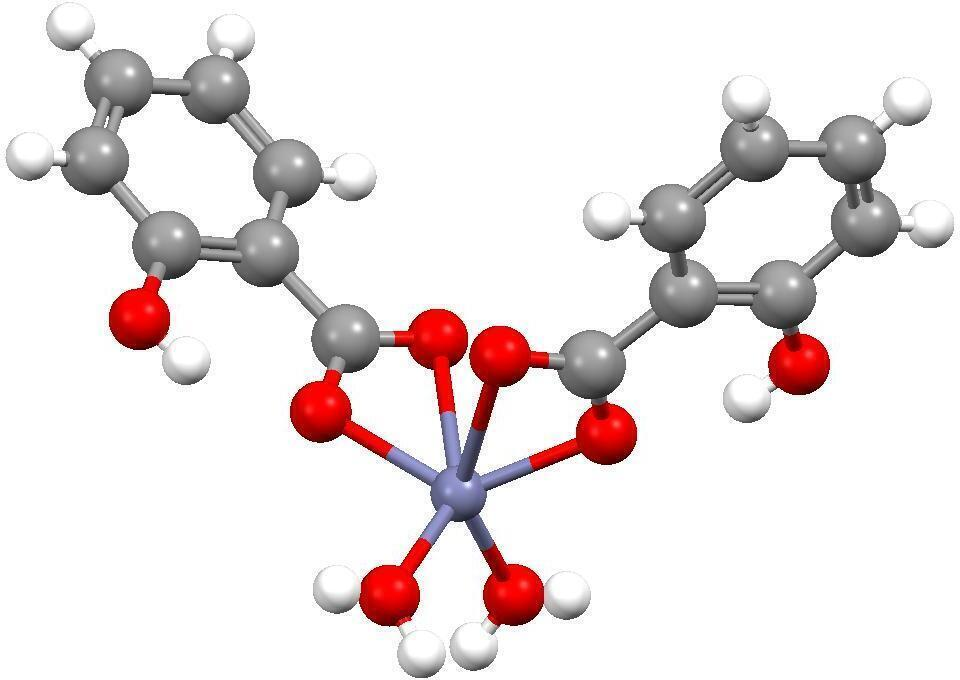
\includegraphics[width=\textwidth]{assets/37}
    \end{subfigure}
    \hfill
    \begin{subfigure}[b]{0.45\textwidth}
        \centering
        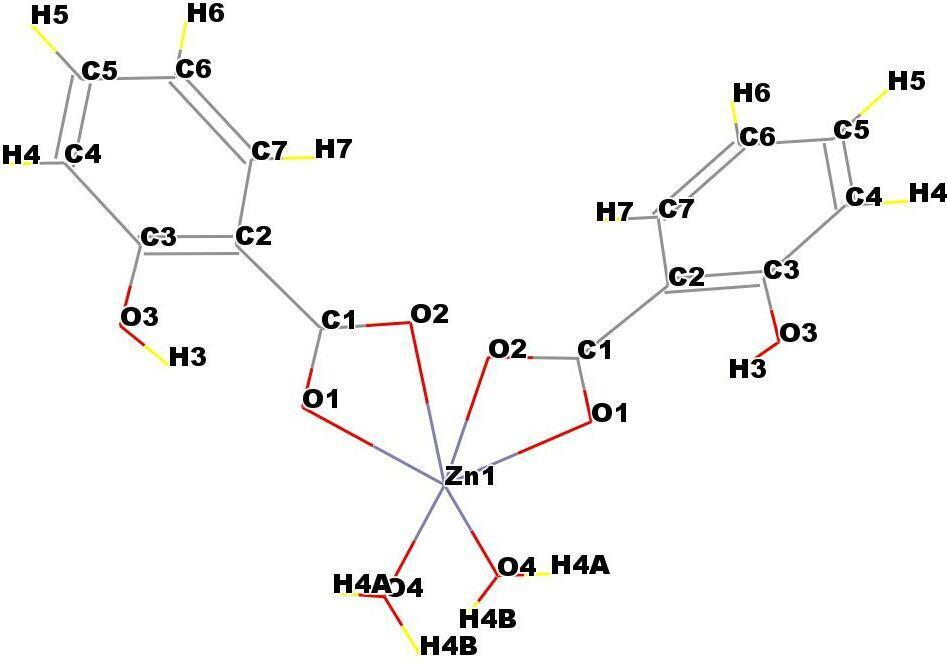
\includegraphics[width=\textwidth]{assets/38}
    \end{subfigure}
    \caption*{Figure 1 - Structural formula of the Zn(HSal)\textsubscript{2}·2H\textsubscript{2}O molecule obtained with X-ray diffraction by Gusev \emph{et al}.}
\end{figure}

\begin{multicols}{2}
The crystal structure of zinc (II) salicylate dihydrate was first
described by Klug {[}31{]}. The thermal behavior of zinc salicylate and
5-chlorosalicylate complexes with bioactive ligands was studied by
Chomič \emph{et al} {[}32,33{]}\emph{.} The stability constant of zinc
(II) salicylate was determined by Singh {[}34{]}.

{\bfseries \emph{Bond length.}} As part of our investigation, we first
presented the PM3-optimized geometry parameters (bond length and angle)
in the gas and aqueous phases in comparison to available X-ray analysis
data. The calculated and experimental values \hspace{0pt}\hspace{0pt}of
the bond lengths are listed in Table 1. The list of atoms corresponds to
Figure 1.

A comparison of the calculated bond lengths of zinc salicylate with
X-ray structural data shows that they agree well in the case of the
aqueous phase. For example, the calculated length of the Zn1-O1 bond is
1.9897Å while the experimental value is 1.9928Å. These values lie within
acceptable deviations. Bond length values
\hspace{0pt}\hspace{0pt}calculated for the gas phase are less consistent
with experimental results. In addition, the calculated bond lengths of
the zinc salicylate molecule in the gas phase are slightly longer than
in aqueous phase. An exception are the Zn(1)-O(4) coordination bonds and
the O-H-bond in coordinated water molecules, whose lengths were
significantly longer for the gas phase.

The lengths of the C=C bonds in the benzene ring are typical for
aromatic compounds. The calculated length also agrees well with the
reference data.

{\bfseries \emph{Bond angles.}} Experimental and calculated values of the
bond angles are listed in Table 2.

A comparison of the results of the PM3 zinc salicylate bond angle
calculations show the same trend as the results of the bond length
calculations. The angle values \hspace{0pt}\hspace{0pt}obtained for the
aqueous phase agree well with the X-ray diffraction results. The
calculation for the gas phase shows a significantly lower correlation to
experimental data. It can be clearly concluded that the best results for
calculating the geometry of such molecules can be obtained for the
solution phase. In this case, gas phase calculations are performed with
significant errors.
\end{multicols}

\begin{table}[H]
\caption*{Table 1 - Comparison between experimental X-ray and PM3 calculated bond lengths (Å) of Zn(HSal)\textsubscript{2}·2H\textsubscript{2}O for the gas and aqueous phases.}
\centering
\begin{tabular}{|l|l|lll|}
\hline
\multirow{2}{*}{Atom 1} & \multirow{2}{*}{Atom 2} & \multicolumn{3}{l|}{Bond length, Å} \\ \cline{3-5} 
 &  & \multicolumn{1}{l|}{XRD data} & \multicolumn{1}{l|}{Gas phase} & Aqueous phase \\ \hline
Zn1 & O1 & \multicolumn{1}{l|}{1.9928} & \multicolumn{1}{l|}{2.1156} & 1.9897 \\ \hline
Zn1 & O2 & \multicolumn{1}{l|}{2.5679} & \multicolumn{1}{l|}{2.3277} & 2.5815 \\ \hline
Zn1 & O4 & \multicolumn{1}{l|}{1.9857} & \multicolumn{1}{l|}{2.3194} & 2.0294 \\ \hline
Zn1 & O1 & \multicolumn{1}{l|}{1.9928} & \multicolumn{1}{l|}{2.1156} & 1.9897 \\ \hline
Zn1 & O2 & \multicolumn{1}{l|}{2.5679} & \multicolumn{1}{l|}{2.2659} & 2.5815 \\ \hline
Zn1 & O4 & \multicolumn{1}{l|}{1.9857} & \multicolumn{1}{l|}{2.3042} & 2.0294 \\ \hline
O1 & C1 & \multicolumn{1}{l|}{1.2830} & \multicolumn{1}{l|}{1.3328} & 1.2651 \\ \hline
O2 & C1 & \multicolumn{1}{l|}{1.2533} & \multicolumn{1}{l|}{1.2584} & 1.2312 \\ \hline
O3 & C3 & \multicolumn{1}{l|}{1.3641} & \multicolumn{1}{l|}{1.3760} & 1.3874 \\ \hline
O3 & H3 & \multicolumn{1}{l|}{0.7692} & \multicolumn{1}{l|}{0.9580} & 0.7716 \\ \hline
O4 & H4A & \multicolumn{1}{l|}{0.6499} & \multicolumn{1}{l|}{0.9452} & 0.6498 \\ \hline
O4 & H4B & \multicolumn{1}{l|}{0.8521} & \multicolumn{1}{l|}{0.9413} & 0.8136 \\ \hline
C1 & C2 & \multicolumn{1}{l|}{1.4796} & \multicolumn{1}{l|}{1.4894} & 1.4682 \\ \hline
C7 & H7 & \multicolumn{1}{l|}{0.9306} & \multicolumn{1}{l|}{1.1000} & 0.9077 \\ \hline
C7 & C2 & \multicolumn{1}{l|}{1.4039} & \multicolumn{1}{l|}{1.3953} & 1.4079 \\ \hline
C7 & C6 & \multicolumn{1}{l|}{1.3806} & \multicolumn{1}{l|}{1.3940} & 1.4053 \\ \hline
C3 & C2 & \multicolumn{1}{l|}{1.4065} & \multicolumn{1}{l|}{1.3394} & 1.3907 \\ \hline
C3 & C4 & \multicolumn{1}{l|}{1.3874} & \multicolumn{1}{l|}{1.4232} & 1.3667 \\ \hline
C5 & H5 & \multicolumn{1}{l|}{0.9303} & \multicolumn{1}{l|}{1.1108} & 0.9208 \\ \hline
C5 & C6 & \multicolumn{1}{l|}{1.3964} & \multicolumn{1}{l|}{1.3451} & 1.3966 \\ \hline
C5 & C4 & \multicolumn{1}{l|}{1.3860} & \multicolumn{1}{l|}{1.3396} & 1.3737 \\ \hline
C6 & H6 & \multicolumn{1}{l|}{0.9305} & \multicolumn{1}{l|}{1.0886} & 0.8965 \\ \hline
C4 & H4 & \multicolumn{1}{l|}{0.9291} & \multicolumn{1}{l|}{1.1186} & 0.8952 \\ \hline
O1 & C1 & \multicolumn{1}{l|}{1.2830} & \multicolumn{1}{l|}{1.3328} & 1.2651 \\ \hline
O2 & C1 & \multicolumn{1}{l|}{1.2532} & \multicolumn{1}{l|}{1.2584} & 1.2312 \\ \hline
O3 & C3 & \multicolumn{1}{l|}{1.3641} & \multicolumn{1}{l|}{1.3760} & 1.3874 \\ \hline
O3 & H3 & \multicolumn{1}{l|}{0.7691} & \multicolumn{1}{l|}{0.9580} & 0.7716 \\ \hline
O4 & H4A & \multicolumn{1}{l|}{0.6499} & \multicolumn{1}{l|}{0.9452} & 0.6498 \\ \hline
O4 & H4B & \multicolumn{1}{l|}{0.8521} & \multicolumn{1}{l|}{0.9413} & 0.8136 \\ \hline
C1 & C2 & \multicolumn{1}{l|}{1.4796} & \multicolumn{1}{l|}{1.4894} & 1.4682 \\ \hline
C7 & H7 & \multicolumn{1}{l|}{0.9306} & \multicolumn{1}{l|}{1.1000} & 0.9077 \\ \hline
C7 & C2 & \multicolumn{1}{l|}{1.4039} & \multicolumn{1}{l|}{1.3953} & 1.4079 \\ \hline
C7 & C6 & \multicolumn{1}{l|}{1.3806} & \multicolumn{1}{l|}{1.3940} & 1.4053 \\ \hline
C3 & C2 & \multicolumn{1}{l|}{1.4065} & \multicolumn{1}{l|}{1.3394} & 1.3907 \\ \hline
C3 & C4 & \multicolumn{1}{l|}{1.3874} & \multicolumn{1}{l|}{1.4232} & 1.3667 \\ \hline
C5 & H5 & \multicolumn{1}{l|}{0.9303} & \multicolumn{1}{l|}{1.1108} & 0.9208 \\ \hline
C5 & C6 & \multicolumn{1}{l|}{1.3964} & \multicolumn{1}{l|}{1.3451} & 1.3966 \\ \hline
C5 & C4 & \multicolumn{1}{l|}{1.3861} & \multicolumn{1}{l|}{1.3396} & 1.3737 \\ \hline
C6 & H6 & \multicolumn{1}{l|}{0.9305} & \multicolumn{1}{l|}{1.0886} & 0.8965 \\ \hline
C4 & H4 & \multicolumn{1}{l|}{0.9292} & \multicolumn{1}{l|}{1.1186} & 0.8952 \\ \hline
\end{tabular}
\end{table}

\begin{table}[H]
\caption{Table 2 - Bond angle properties of Zn(HSal)\textsubscript{2}·2H\textsubscript{2}O obtained from XRD and calculated using the PM3 method.}
\centering
\begin{tabular}{|l|l|l|lll|}
\hline
\multirow{2}{*}{Atom 1*} & \multirow{2}{*}{Atom 2*} & \multirow{2}{*}{Atom 3*} & \multicolumn{3}{l|}{Bond 				angle (deg)} \\ \cline{4-6} 
 &  &  & \multicolumn{1}{l|}{XRD data} & \multicolumn{1}{l|}{Gas phase} & Aqueous phase \\ \hline
O1 & Zn1 & O2 & \multicolumn{1}{l|}{56.03} & \multicolumn{1}{l|}{57.27} & 55.07 \\ \hline
O1 & Zn1 & O4 & \multicolumn{1}{l|}{120.11} & \multicolumn{1}{l|}{112.40} & 119.68 \\ \hline
O1 & Zn1 & O1 & \multicolumn{1}{l|}{128.18} & \multicolumn{1}{l|}{145.40} & 127.48 \\ \hline
O1 & Zn1 & O2 & \multicolumn{1}{l|}{86.98} & \multicolumn{1}{l|}{99.58} & 85.12 \\ \hline
O1 & Zn1 & O4 & \multicolumn{1}{l|}{92.86} & \multicolumn{1}{l|}{91.74} & 90.46 \\ \hline
O2 & Zn1 & O4 & \multicolumn{1}{l|}{91.72} & \multicolumn{1}{l|}{90.81} & 90.85 \\ \hline
O2 & Zn1 & O1 & \multicolumn{1}{l|}{86.98} & \multicolumn{1}{l|}{99.90} & 85.12 \\ \hline
O2 & Zn1 & O2 & \multicolumn{1}{l|}{91.21} & \multicolumn{1}{l|}{99.56} & 90.54 \\ \hline
O2 & Zn1 & O4 & \multicolumn{1}{l|}{148.53} & \multicolumn{1}{l|}{147.68} & 147.65 \\ \hline
O4 & Zn1 & O1 & \multicolumn{1}{l|}{92.86} & \multicolumn{1}{l|}{88.28} & 90.46 \\ \hline
O4 & Zn1 & O2 & \multicolumn{1}{l|}{148.53} & \multicolumn{1}{l|}{143.73} & 147.65 \\ \hline
O4 & Zn1 & O4 & \multicolumn{1}{l|}{101.74} & \multicolumn{1}{l|}{91.92} & 101.00 \\ \hline
O1 & Zn1 & O2 & \multicolumn{1}{l|}{56.03} & \multicolumn{1}{l|}{57.27} & 55.07 \\ \hline
O1 & Zn1 & O4 & \multicolumn{1}{l|}{120.11} & \multicolumn{1}{l|}{114.71} & 119.68 \\ \hline
O2 & Zn1 & O4 & \multicolumn{1}{l|}{91.72} & \multicolumn{1}{l|}{94.38} & 90.85 \\ \hline
Zn1 & O1 & C1 & \multicolumn{1}{l|}{104.47} & \multicolumn{1}{l|}{98.21} & 104.94 \\ \hline
Zn1 & O2 & C1 & \multicolumn{1}{l|}{78.62} & \multicolumn{1}{l|}{91.07} & 77.49 \\ \hline
C3 & O3 & H3 & \multicolumn{1}{l|}{106.76} & \multicolumn{1}{l|}{107.91} & 104.75 \\ \hline
Zn1 & O4 & H4A & \multicolumn{1}{l|}{114.69} & \multicolumn{1}{l|}{100.15} & 111.15 \\ \hline
Zn1 & O4 & H4B & \multicolumn{1}{l|}{120.35} & \multicolumn{1}{l|}{102.46} & 120.99 \\ \hline
H4A & O4 & H4B & \multicolumn{1}{l|}{122.19} & \multicolumn{1}{l|}{101.98} & 121.35 \\ \hline
O1 & C1 & O2 & \multicolumn{1}{l|}{120.46} & \multicolumn{1}{l|}{111.12} & 121.99 \\ \hline
O1 & C1 & C2 & \multicolumn{1}{l|}{118.01} & \multicolumn{1}{l|}{121.43} & 117.24 \\ \hline
O2 & C1 & C2 & \multicolumn{1}{l|}{121.51} & \multicolumn{1}{l|}{121.71} & 120.72 \\ \hline
H7 & C7 & C2 & \multicolumn{1}{l|}{119.30} & \multicolumn{1}{l|}{119.59} & 118.93 \\ \hline
H7 & C7 & C6 & \multicolumn{1}{l|}{119.30} & \multicolumn{1}{l|}{120.93} & 119.60 \\ \hline
C2 & C7 & C6 & \multicolumn{1}{l|}{121.40} & \multicolumn{1}{l|}{120.25} & 119.55 \\ \hline
O3 & C3 & C2 & \multicolumn{1}{l|}{121.63} & \multicolumn{1}{l|}{123.88} & 121.59 \\ \hline
O3 & C3 & C4 & \multicolumn{1}{l|}{117.81} & \multicolumn{1}{l|}{128.18} & 117.40 \\ \hline
C2 & C3 & C4 & \multicolumn{1}{l|}{120.56} & \multicolumn{1}{l|}{120.39} & 120.88 \\ \hline
C1 & C2 & C7 & \multicolumn{1}{l|}{120.06} & \multicolumn{1}{l|}{120.34} & 120.28 \\ \hline
C1 & C2 & C3 & \multicolumn{1}{l|}{121.64} & \multicolumn{1}{l|}{120.60} & 121.20 \\ \hline
C7 & C2 & C3 & \multicolumn{1}{l|}{118.23} & \multicolumn{1}{l|}{119.44} & 118.47 \\ \hline
H5 & C5 & C6 & \multicolumn{1}{l|}{119.70} & \multicolumn{1}{l|}{119.83} & 117.08 \\ \hline
H5 & C5 & C4 & \multicolumn{1}{l|}{119.72} & \multicolumn{1}{l|}{119.37} & 119.23 \\ \hline
C6 & C5 & C4 & \multicolumn{1}{l|}{120.58} & \multicolumn{1}{l|}{116.83} & 121.68 \\ \hline
C7 & C6 & C5 & \multicolumn{1}{l|}{119.26} & \multicolumn{1}{l|}{120.35} & 118.71 \\ \hline
C7 & C6 & H6 & \multicolumn{1}{l|}{120.34} & \multicolumn{1}{l|}{119.77} & 119.83 \\ \hline
C5 & C6 & H6 & \multicolumn{1}{l|}{120.40} & \multicolumn{1}{l|}{116.49} & 120.69 \\ \hline
C3 & C4 & C5 & \multicolumn{1}{l|}{119.96} & \multicolumn{1}{l|}{129.69} & 118.94 \\ \hline
C3 & C4 & H4 & \multicolumn{1}{l|}{120.00} & \multicolumn{1}{l|}{119.77} & 120.06 \\ \hline
C5 & C4 & H4 & \multicolumn{1}{l|}{120.04} & \multicolumn{1}{l|}{114.33} & 120.96 \\ \hline
Zn1 & O1 & C1 & \multicolumn{1}{l|}{104.47} & \multicolumn{1}{l|}{96.94} & 104.96 \\ \hline
Zn1 & O2 & C1 & \multicolumn{1}{l|}{78.62} & \multicolumn{1}{l|}{98.38} & 77.49 \\ \hline
C3 & O3 & H3 & \multicolumn{1}{l|}{106.77} & \multicolumn{1}{l|}{106.71} & 104.75 \\ \hline
Zn1 & O4 & H4A & \multicolumn{1}{l|}{114.69} & \multicolumn{1}{l|}{102.46} & 111.15 \\ \hline
\end{tabular}
\end{table}

\begin{table}[H]
\centering
\begin{tabular}{|l|l|l|lll|}
\hline
\multirow{2}{*}{Atom 1*} & \multirow{2}{*}{Atom 2*} & \multirow{2}{*}{Atom 3*} & \multicolumn{3}{l|}{Bond 				angle (deg)} \\ \cline{4-6} 
 &  &  & \multicolumn{1}{l|}{XRD data} & \multicolumn{1}{l|}{Gas phase} & Aqueous phase \\ \hline
Zn1 & O4 & H4B & \multicolumn{1}{l|}{120.34} & \multicolumn{1}{l|}{100.65} & 120.99 \\ \hline
H4A & O4 & H4B & \multicolumn{1}{l|}{122.20} & \multicolumn{1}{l|}{108.95} & 121.35 \\ \hline
O1 & C1 & O2 & \multicolumn{1}{l|}{120.46} & \multicolumn{1}{l|}{111.12} & 121.99 \\ \hline
O1 & C1 & C2 & \multicolumn{1}{l|}{118.01} & \multicolumn{1}{l|}{121.30} & 117.24 \\ \hline
O2 & C1 & C2 & \multicolumn{1}{l|}{121.51} & \multicolumn{1}{l|}{121.71} & 120.72 \\ \hline
H7 & C7 & C2 & \multicolumn{1}{l|}{119.30} & \multicolumn{1}{l|}{119.41} & 118.93 \\ \hline
H7 & C7 & C6 & \multicolumn{1}{l|}{119.30} & \multicolumn{1}{l|}{122.79} & 119.60 \\ \hline
C2 & C7 & C6 & \multicolumn{1}{l|}{121.40} & \multicolumn{1}{l|}{120.46} & 119.55 \\ \hline
O3 & C3 & C2 & \multicolumn{1}{l|}{121.63} & \multicolumn{1}{l|}{124.63} & 121.59 \\ \hline
O3 & C3 & C4 & \multicolumn{1}{l|}{117.81} & \multicolumn{1}{l|}{128.18} & 117.40 \\ \hline
C2 & C3 & C4 & \multicolumn{1}{l|}{120.56} & \multicolumn{1}{l|}{120.21} & 120.88 \\ \hline
C1 & C2 & C7 & \multicolumn{1}{l|}{120.06} & \multicolumn{1}{l|}{120.55} & 120.28 \\ \hline
C1 & C2 & C3 & \multicolumn{1}{l|}{121.64} & \multicolumn{1}{l|}{120.29} & 121.20 \\ \hline
C7 & C2 & C3 & \multicolumn{1}{l|}{118.23} & \multicolumn{1}{l|}{119.44} & 118.47 \\ \hline
H5 & C5 & C6 & \multicolumn{1}{l|}{119.70} & \multicolumn{1}{l|}{119.56} & 117.08 \\ \hline
H5 & C5 & C4 & \multicolumn{1}{l|}{119.72} & \multicolumn{1}{l|}{123.61} & 119.23 \\ \hline
C6 & C5 & C4 & \multicolumn{1}{l|}{120.57} & \multicolumn{1}{l|}{116.83} & 121.68 \\ \hline
C7 & C6 & C5 & \multicolumn{1}{l|}{119.26} & \multicolumn{1}{l|}{120.37} & 118.71 \\ \hline
C7 & C6 & H6 & \multicolumn{1}{l|}{120.34} & \multicolumn{1}{l|}{119.72} & 119.83 \\ \hline
C5 & C6 & H6 & \multicolumn{1}{l|}{120.39} & \multicolumn{1}{l|}{121.05} & 120.69 \\ \hline
C3 & C4 & C5 & \multicolumn{1}{l|}{119.96} & \multicolumn{1}{l|}{119.70} & 118.94 \\ \hline
C3 & C4 & H4 & \multicolumn{1}{l|}{120.00} & \multicolumn{1}{l|}{119.43} & 120.06 \\ \hline
C5 & C4 & H4 & \multicolumn{1}{l|}{120.04} & \multicolumn{1}{l|}{121.11} & 120.96 \\ \hline
\multicolumn{6}{|l|}{* - \emph{numbering of atoms is in accordance with Fig.1.}} \\ \hline
\end{tabular}
\end{table}

\begin{multicols}{2}
\emph{{\bfseries Mulliken charges population analysis.}} The local
reactivity of zinc salicylate was studied using Mulliken charge
population analysis, which provides an indication of the reactive
(nucleophilic and electrophilic) centers of molecules. Therefore, the
regions of the molecule with high electronic charge are chemically
softer than the regions with low electronic charge, so electron density
plays an important role in chemical reactivity calculations. The results
of the Mulliken atomic charge calculation are shown in Figure 2.
\end{multicols}

\begin{figure}[H]
    \centering
    \begin{subfigure}[b]{0.45\textwidth}
        \centering
        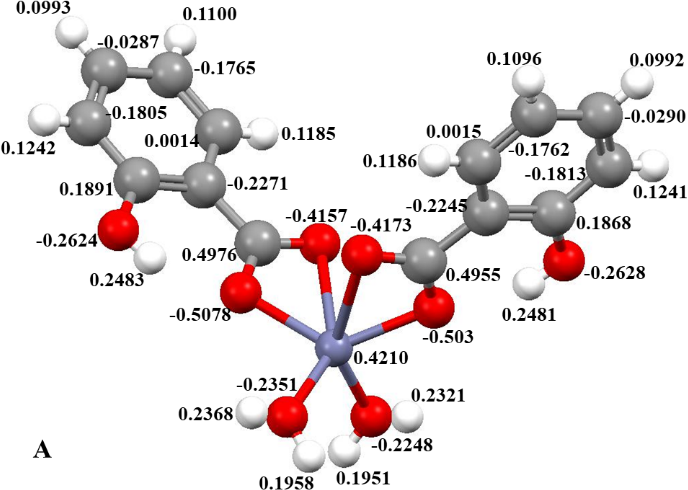
\includegraphics[width=\textwidth]{assets/39}
    \end{subfigure}
    \hfill
    \begin{subfigure}[b]{0.45\textwidth}
        \centering
        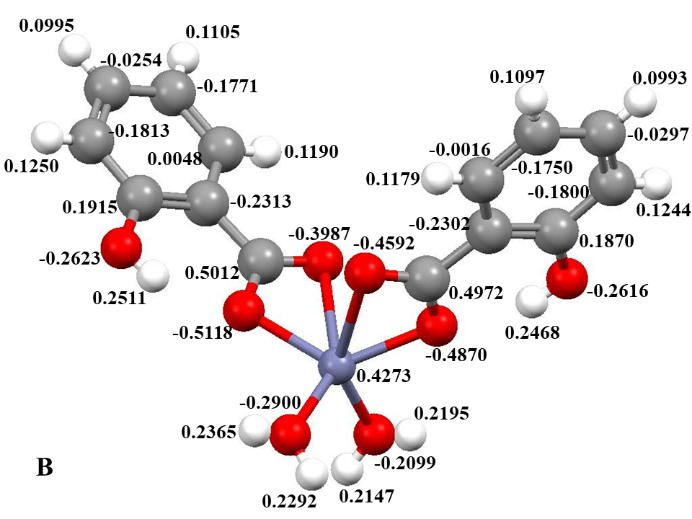
\includegraphics[width=\textwidth]{assets/40}
    \end{subfigure}
    \caption*{Figure 2 - PM3 Mulliken charges population for the calculated Zn(HSal)\textsubscript{2}·2H\textsubscript{2}O molecule in gas (A) and aqueous (B) phase.}
\end{figure}

\begin{multicols}{2}
The place for a nucleophilic attack is where the value of the positive
charge is maximum. The location of electrophilic attack is in turn
controlled by the negative charge value. Mulliken charge population
analysis shows that the zinc atoms in both the gas and aqueous phases
have the maximum positive charge. The most negative charges are on the
oxygen atoms of the carboxyl groups. Consequently, the oxygen atoms of
the carboxyl groups are most susceptible to electrophilic attack. The
presence of water leads to a slight shift in the electron density
towards the oxygen atoms of the carboxyl groups, which becomes more
negative.

\emph{{\bfseries Frontier molecular orbitals (FMO).}} Frontier orbital
theory is very useful for determining the main properties of molecules.
The positions of the highest occupied molecular orbital (HOMO) and the
lowest unoccupied molecular orbital (LUMO) are molecular parameters that
are directly related to the electron and hole transport properties of
the substance. The energy gap value (ΔE\textsubscript{gap}) is the
difference between HOMO-LUMO and is used as a significant descriptor of
molecular stability. The most stable molecule has a low
ΔE\textsubscript{gap}.

The molecular electrostatic potential (MEP), frontier molecular orbitals
energies and ΔE\textsubscript{gap} calculated for
Zn(HSal)\textsubscript{2}·2H\textsubscript{2}O are shown in Figure 3.
\end{multicols}

\begin{figure}[H]
	\centering
	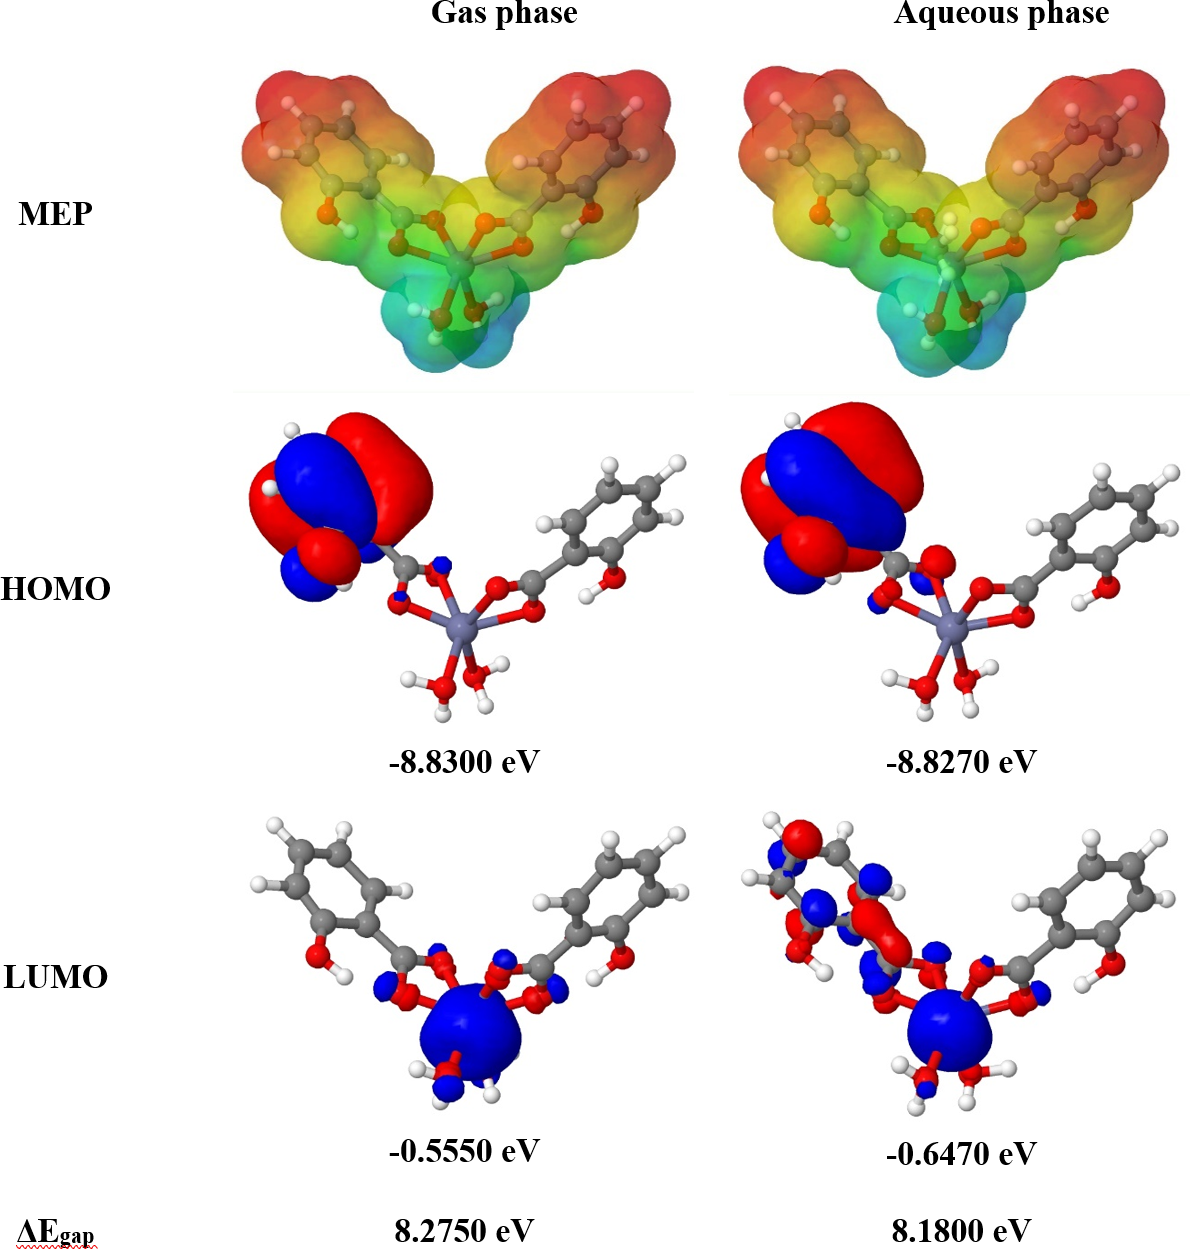
\includegraphics[width=0.8\textwidth]{assets/41}
	\caption*{Figure 3 - The molecular electrostatic potential (MEP) and frontier molecular orbitals (HOMO-LUMO) density distribution of the Zn(HSal)\textsubscript{2}·2H\textsubscript{2}O calculated with PM3 for gas and aqueous phases.}
\end{figure}

\begin{multicols}{2}
The positively charged lobe is indicated by the blue color, and the
negatively charged lobe is indicated by the red color.

E\textsubscript{HOMO} describes the electron donating ability of the
molecule. Conversely, E\textsubscript{LUMO} describes the ability of the
molecule to accept electrons. The lower the LUMO value, the higher the
ability of the compound to accept electrons. The HOMOs of
Zn(HSal)\textsubscript{2}·2H\textsubscript{2}O are mainly located at the
oxygen atoms of the -OH-group in the ortho-position. On the other hand,
the LUMOs are mainly located on the zinc atoms and oxygen atoms of the
carboxyl units. The presence of water as a high dielectric constant
model solvent results in a slight decrease in the LUMO energy (around
0.095 eV) and a non-significant decrease in the HOMO energy.

Negative values for E\textsubscript{HOMO} and E\textsubscript{LUMO}
indicate the presence of additional electron pairs in both the upper and
lower molecular orbitals. This means that zinc salicylate should act as
an electron donor in chemical transformations. A low negative LUMO value
(near zero) indicates that zinc salicylate is a weak electrophile.

The gap energy (ΔE\textsubscript{gap}, Eq.1.) between the frontier
orbitals is usually of great importance in describing static molecular
reactivity. Large energy gap values \hspace{0pt}\hspace{0pt}mean high
electronic stability and therefore low reactivity. In the gas phase,
zinc salicylate has a higher ΔE\textsubscript{gap} value than in
solution (8.275 eV and 8.180 eV respectively). Therefore, zinc
salicylate is more stable in the gas phase than in solution. Under the
influence of polar water molecules, zinc salicylate becomes unstable as
it dissolves and dissociates into ions.

{\bfseries \emph{Quantum chemical descriptors.}} In accordance with the
relationship of HOMO-LUMO energy values, the reactivity descriptors of
the Zn(HSal)\textsubscript{2}·2H\textsubscript{2}O molecule were
calculated using formulas 2-8 in gas and aqueous phases. The calculation
results obtained are shown in Table 3.
\end{multicols}


\begin{table}[H]
\caption*{Table 3 - Quantum chemical descriptors of the Zn(HSal)\textsubscript{2}·2H\textsubscript{2}O molecule calculated using the PM3 method in the gas and aqueous phase.}
\centering
\begin{tabular}{|l|l|l|}
\hline
Descriptor & Gas phase & Aqueous phase \\ \hline
Heat of formation (ΔHf), kJ/mol & -1079.97 & -1102.20 \\ \hline
Dipole moment (μ), D & 4.9320 & 3.9620 \\ \hline
Ionization energy (IP), eV & 8.8300 & 8.8270 \\ \hline
Electron affinity (EA), eV & 0.5550 & 0.6470 \\ \hline
Electronegativity (χ), eV & 4.6925 & 4.7370 \\ \hline
Chemical hardness (η), eV & 4.1375 & 4.0900 \\ \hline
Chemical softness (σ), eV & 0.2417 & 0.2445 \\ \hline
Electrophilicity index (ω), eV & 2.6610 & 2.7432 \\ \hline
Nucleophilicity index (ε), eV & 0.3758 & 0.3645 \\ \hline
\end{tabular}
\end{table}

The heat of formation value provides a quantitative estimate of the
energy required to destroy the molecule. The negative value of the heat
of formation indicates the high stability of the substance both in the
gas phase (-1079.97 kJ/mol) and in the aqueous phase (-1102.97 kJ/mol).
A more negative value indicates greater stability of zinc salicylate in
the aqueous phase. PM3 predicts these values for a standard
thermodynamic temperature of 298.15 K.

Comparison of the calculated dipole moment (μ) of zinc salicylate
(4,9320 D gas, 3.9620 D aqueous) with the dipole moments of water (1.83
D) and alcohols (CH\textsubscript{3}OH 1.69 D,
C\textsubscript{2}H\textsubscript{5}OH 1.66 D) shows its good solubility
in polar solvents, especially in water. Dipole moment values also show
that zinc salicylate readily dissolves in aprotic polar solvents such as
dimethylacetamide (3.72 D), N,N-dimethylformamide (3.86 D),
N-methylpyrrolidone (4.09 D), dimethyl sulfoxide (4.1 D) and propylene
carbonate (4.94 D). Zinc salicylate should be insoluble in non-polar
solvents.

Electronegativity indicates the molecular ability to accept electrons.
The structure obtained in the aqueous phase becomes more electronegative
than in the gas phase. Value of global hardness (η) based on 4.137 eV
and 4.09 eV for the gas and aqueous phases, respectively. This means
that zinc salicylate is a hard reagent in both phases and a better
electrophile in the aqueous phase.

The global softness (σ) is the reciprocal of the global hardness
{[}35{]}. Both are related to the principle of hard and soft acid and
base (HSAB) and are very useful in explaining various experimental
observations. These parameters characterize the molecule as a whole.
Softness is an important property for measuring the molecular stability
and reactivity. The calculated softness value for zinc salicylate is
higher in aqueous than in the gas phase.

The global electrophilicity index (ω) introduced by Parr {[}36,37{]}, is
a measure of energy stabilization after a molecule has acquired an
additional amount of electrons. As shown in Table 3, zinc salicylate has
the highest value of electrophilicity index in the aqueous phase.
Therefore, zinc salicylate is chemically more reactive in the gas phase.

{\bfseries Conclusion.} In this research,
Zn(HSal)\textsubscript{2}·2H\textsubscript{2}O was studied using the
semi-empirical PM3 computational approach. The calculations were carried
out for the gas and aqueous phases. The calculations performed in the
present study predict that the calculated geometric parameters are close
to those from X-ray studies. A comparison of the available X-ray
crystallographic data and the theoretical results obtained shows that
there is a large correlation. The best agreement was found for the
aqueous phase calculations. PM3 calculation of the geometry of zinc
salicylate dihydrate performs quite well in terms of both bond distances
and bond angles. The agreement between calculated and experimental data
is satisfactory, especially in the case of the aqueous phase
calculation. Therefore, this approach is promising for application to
such systems.

{\bfseries References}

\begin{enumerate}
\def\labelenumi{\arabic{enumi}.}
\item
  Das S. K. et al. Highly porous Co (II)-salicylate metal--organic
  framework: synthesis, characterization and magnetic properties
  //Dalton Transactions. -- 2011. -- Vol. 40 (12) -- P. 2932-2939.
  https://doi.org/10.1039/C0DT01483D
\item
  Kohno Y. \emph{et al.} A cobalt (II) bis (salicylate)-based ionic
  liquid that shows thermoresponsive and selective water coordination
  //Chemical Communications. -- 2014. -- Vol. 50 (50) -- P. 6633-6636.
  https://doi:10.1039/c4cc01023j
\item
  Chakraborty B., Paine T. K. Synthesis and characterization of cobalt
  (II)--salicylate complexes derived from N4-donor ligands:
  Stabilization of a hexameric water cluster in the lattice host of a
  cobalt (III)--salicylate complex //Inorganica Chimica Acta. -- 2011.
  -- Vol. 378 (1) -- P. 231-238.
  https://doi.org/10.1016/j.ica.2011.09.008
\item
  Devereux M. \emph{et al}. Manganese (II) salicylate complexes as
  H\textsubscript{2}O\textsubscript{2} disproportionation catalysts:
  X-ray crystal structure of {[}Mn(Hsal)\textsubscript{2}
  (bipy){]}·H\textsubscript{2}O (H\textsubscript{2}sal= salicylic acid,
  bipy= 2,2′-bipyridine) //Polyhedron. -- 1996. -- Vol. 15 (12) -- P.
  2029-2033. https://doi.org/10.1016/0277-5387(95)00452-1
\item
  Lemoine P. \emph{et al.} Crystal structure of bis
  (N,N-dimethylbiguanide) nickel (II) salicylate,
  C\textsubscript{22}H\textsubscript{32}N\textsubscript{10}NiO\textsubscript{6}
  //Zeitschrift für Kristallographie-New Crystal Structures. -- 1999. --
  Vol. 214 (3) -- P. 369-370. https://doi.org/10.1515/ncrs-1999-0337
\item
  Jian F. \emph{et al}. Structure of hexakis (imidazole) nickel (II)
  disalicylate,{[}Ni(Im)\textsubscript{6}{]}(Sal)\textsubscript{2}
  //Journal of chemical crystallography. -- 1999. -- Vol. 29. -- P.
  359-363. https://doi.org/10.1023/A:1009542422416
\item
  Auer D. E., Ng J. C., Seawright A. A. Copper salicylate and copper
  phenylbutazone as topically applied anti‐inflammatory agents in the
  rat and horse //Journal of Veterinary Pharmacology and Therapeutics.
  -- 1990. -- Vol (1) -- P. 67-75.
  https://doi.org/10.1111/j.1365-2885.1990.tb00749.x
\item
  Ünaleroǧlu C., Zümreoǧlu-Karan B., Mert Y. Zinc ascorbate: a combined
  experimental and computational study for structure elucidation
  //Journal of molecular structure. -- 2002. -- Vol. 605 (2-3) -- P.
  227-233. https://doi.org/10.1016/S0022-2860(01)00765-7
\item
  Lansdown A. B. G. \emph{et al}. Zinc in wound healing: theoretical,
  experimental, and clinical aspects //Wound repair and regeneration. --
  2007. -- Vol. 15 (1) -- P. 2-16.
  https://doi.org/10.1111/j.1524-475X.2006.00179.x
\item
  Lin P. H. \emph{et al.} Zinc in wound healing modulation //Nutrients.
  -- 2017. -- Vol. 10 (1) -- P. 16. https://doi.org/10.3390/nu10010016
\item
  Scrimshaw N. S., Young V. R. The requirements of human nutrition
  //Scientific American. -- 1976. -- Vol. 235 (3) -- P. 50-65.
  http://www.jstor.org/stable/24950435
\item
  Cabot C. \emph{et al}. A role for zinc in plant defense against
  pathogens and herbivores //Frontiers in plant science. -- 2019. --
  Vol. 10. -- P. 1171. https://doi.org/10.3389/fpls.2019.01171
\item
  Balafrej H. et al. Zinc hyperaccumulation in plants: A review
  //Plants. -- 2020. -- Vol. 9 (5) -- P. 562.
  https://doi.org/10.3390/plants9050562
\item
  Bellotti N., Romagnoli R. Assessment of zinc salicylate as antifouling
  product for marine coatings //Industrial \& Engineering Chemistry
  Research. -- 2014. -- Vol. 53 (38) -- P. 14559-14564.
  https://doi.org/10.1021/ie5015734
\item
  Fang L. \emph{et al}. Zinc salicylate reduces airway smooth muscle
  cells remodelling by blocking mTOR and activating
  p21\textsuperscript{(Waf1/Cip1)} //The Journal of Nutritional
  Biochemistry. -- 2021. -- Vol. 89. -- P. 108563.
  https://doi.org/10.1016/j.jnutbio.2020.108563
\item
  Zhang Z. J. et al. Conversion of a zinc salicylate complex into porous
  carbons through a template carbonization process as a superior
  electrode material for supercapacitors //RSC advance. -- 2014. -- Vol.
  4 (13) -- P. 6664-6671. https://doi.org/10.1039/C3RA44981E
\item
  Brownless N. J., Edwards D. A., Mahon M. F. Some complexes derived
  from zinc salicylate or 3, 5-di-tert-butylsalicylate. The crystal
  structure of (2,2′-bipyridyl)(methanol)(O-salicylato)(O,O′-salicylato)
  zinc //Inorganica chimica acta. -- 1999. -- Vol. 287 (1) -- P. 89-94.
  https://doi.org/10.1016/S0020-1693(98)00421-6
\item
  Chooset S. \emph{et al}. Synthesis, crystal structure, luminescent
  properties and antibacterial activities of zinc complexes with
  bipyridyl and salicylate ligands //Inorganica Chimica Acta. -- 2018.
  -- Vol. 471. -- P. 493-501.
  https://doi.org/10.1016/j.ica.2017.11.053Get rights and content
\item
  Mohr M. \emph{et al}. The use of methods involving semi-empirical
  molecular orbital theory to study the structure and reactivity of
  transition metal complexes //Faraday Discussions. -- 2003. -- Vol.
  124. -- P. 413-428. https://doi.org/10.1039/B211791F
\item
  Cundari T. R., Deng J. PM3 (tm) Analysis of Transition-Metal Complexes
  //Journal of chemical information and computer sciences. -- 1999. --
  Vol. 39 (2) -- P. 376-381. https://doi.org/10.1021/ci980145d
\item
  Bosque R., Maseras F. Performance of the semiempirical PM3 (tm) method
  in the geometry optimization of transition metal complexes //Journal
  of Computational Chemistry. -- 2000. -- Vol. 21 (7) -- P. 562-571.
  https://doi.org/10.1002/(SICI)1096-987X(200005)21:7\textless562::AID-JCC5\textgreater3.0.CO;2-0
\item
  Bräuer M. \emph{et al}. Evaluation of the accuracy of PM3, AM1 and
  MNDO/d as applied to zinc compounds //Journal of Molecular Structure:
  THEOCHEM. -- 2000. -- Vol. 505 (1-3) -- P. 289-301.
  https://doi.org/10.1016/S0166-1280(99)00401-7
\item
  Schmidt M. W. \emph{et al}. General atomic and molecular electronic
  structure system //Journal of computational chemistry. -- 1993. --
  Vol. 14 (11) -- P. 1347-1363. https://doi.org/10.1002/jcc.540141112
\item
  Hanwell M. D. \emph{et al.} Avogadro: an advanced semantic chemical
  editor, visualization, and analysis platform //Journal of
  cheminformatics. -- 2012. -- Vol. 4. -- P. 1-17.
  https://doi.org/10.1186/1758-2946-4-17
\item
  Jmol: an open-source Java viewer for chemical structures in 3D
  {[}Electronic source{]}. Available at: http://www.jmol.org.
\item
  Stewart J. J. P. Optimization of parameters for semiempirical methods
  II. Applications //Journal of computational chemistry. -- 1989. --
  Vol. 10 (2) -- P. 221-264. https://doi.org/10.1002/jcc.540100209
\item
  Pinheiro P. S. M. \emph{et al}. Modeling zinc‐oxygen coordination in
  histone deacetylase: a comparison of semiempirical methods performance
  //International Journal of Quantum Chemistry. -- 2018. -- Vol. 118
  (21) -- P. e25720. https://doi.org/10.1002/qua.25720
\item
  Zhan C. G., Nichols J. A., Dixon D. A. Ionization potential, electron
  affinity, electronegativity, hardness, and electron excitation energy:
  molecular properties from density functional theory orbital energies
  //The Journal of Physical Chemistry A. -- 2003. -- Vol. 107 (20) -- P.
  4184-4195. https://doi.org/10.1021/jp0225774
\item
  El Mehdi B. \emph{et al}. Synthesis and comparative study of the
  inhibitive effect of some new triazole derivatives towards corrosion
  of mild steel in hydrochloric acid solution //Materials Chemistry and
  Physics. -- 2003. -- Vol. 77 (2) -- P. 489-496.
  https://doi.org/10.1016/S0254-0584(02)00085-8
\item
  Gusev A. \emph{et al}. Mn (II), Co (II), Ni (II) and Zn salicylates:
  Synthesis, structure and biological properties studies //Inorganica
  Chimica Acta. -- 2021. -- Vol. 528. -- P. 120606.
  https://doi.org/10.1016/j.ica.2021.120606
\item
  Klug H. P., Alexander L. E., Sumner G. G. The crystal structure of
  zinc salicylate dihydrate //Acta Crystallographica. -- 1958. -- Vol.
  11 (1) -- P. 41-46. https://doi.org/10.1107/S0365110X58000086
\item
  Chomič J. \emph{et al}. Thermal study of zinc (II) salicylate complex
  compounds with bioactive ligands //Journal of thermal analysis and
  calorimetry. -- 2004. -- Vol. 76. -- P. 33-41.
  https://doi.org/10.1023/B:JTAN.0000027800.14514.c2
\item
  Györyovő K., Chomič J., Kovőčovő J. Thermal behaviour of zinc (II)
  5-chlorosalicylate complex compounds //Journal of thermal analysis and
  calorimetry. -- 2005. -- Vol. 80. -- P. 375-380.
  https://doi.org/10.1007/s10973-005-0663-0
\item
  Singh R. K. P. \emph{et al}. Stability constants of salicylate of zinc
  (II), cobalt (II), uranyl (II) and thorium (IV) by paper
  electrophoresis //Zeitschrift für Physikalische Chemie. -- 1983. --
  Vol. 264 (1) -- P. 464-468. https://doi.org/10.1515/zpch-1983-26457
\item
  Pearson R. G. Absolute electronegativity and hardness: application to
  inorganic chemistry //Inorganic chemistry. -- 1988. -- Vol. 27 (4) --
  P. 734-740. https://doi.org/10.1021/ic00277a030
\item
  Parr R. G., Pearson R. G. Absolute hardness: companion parameter to
  absolute electronegativity //Journal of the American chemical society.
  -- 1983. -- Vol. 105 (26) -- P. 7512-7516.
  https://doi.org/10.1021/ja00364a005
\item
  Parr R. G., Szentpály L., Liu S. Electrophilicity index //Journal of
  the American Chemical Society. -- 1999. -- Vol. 121 (9) -- P.
  1922-1924. https://doi.org/10.1021/ja983494x
\end{enumerate}

\emph{{\bfseries Information about the authors}}

Akatyev N. V. - Candidate of Chemical Sciences, senior lecturer, M.
Utemisov West Kazakhstan University, Uralsk, Kazakhstan,
e-mail:nikolay.akatyev@wku.edu.kz

\emph{{\bfseries Сведения об авторе}}

Акатьев Н. В. - кандидат химических наук, старший преподаватель,
Западно-Казахстанский университет им. М.Утемисова, Уральск, Казахстан,
e-mail:nikolay.akatyev@wku.edu.kz
